\subsection{Pålitlighet}

\centerline{\textbf{Hur viktigt är pålitlighet för 
din användarupplevelse}}
\begin{figure}[H]
  \centering
  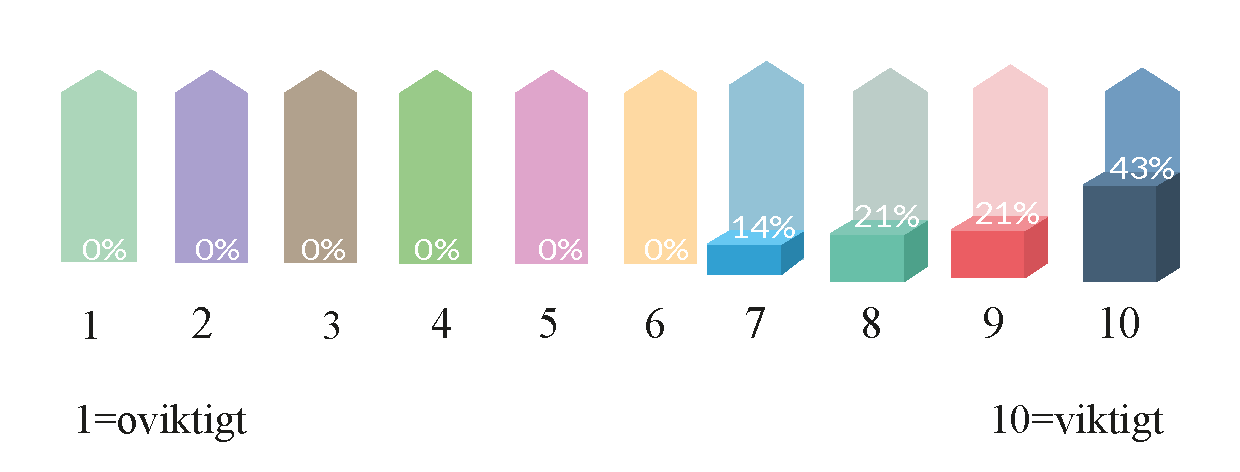
\includegraphics[scale=0.7]{Rityta_13.pdf}
  \centering
  \captionsetup{justification=centering,margin=2cm}
  \caption{Resultat i procentuell skala på respondenternas svar}
\end{figure} 

Medelvärdet av ovan figur är 8.93. Siffran representerar ett medelsnitt av stapeldiagrammet som visar hur viktigt det var för användarupplevelsen enligt kategoriseringen framtagen av  Laugwitz et al. \cite{Laugwitz2008ConstructionQuestionnaire}. 

%\[
%  m = \frac{14+ 24 + 27 + 60}{14} = 8.93
 % \]
  
%Med en standardavvikelse på

%\[
 %  \sigma = \sqrt{V} = \sqrt{  \frac{(7-2)^{2} + (8-3)^{2} + (9-3)^{2} + (10-6)^{2}} {4}} = \sqrt{25.5} = 5.1
  %  \]
\newpage   
\begin{figure}[H]
  \centering
  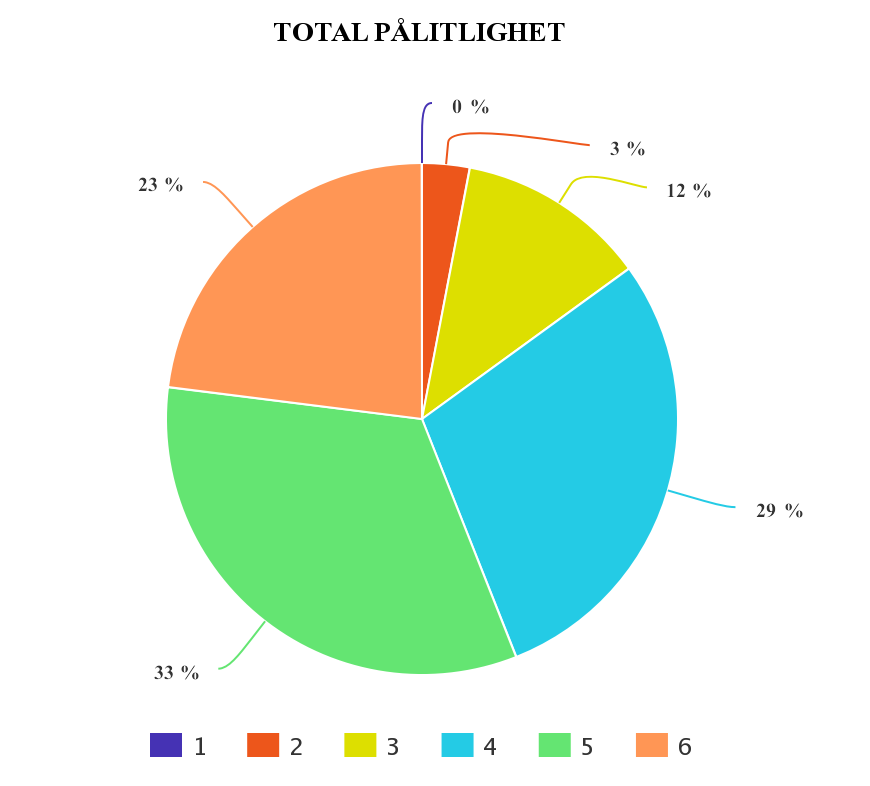
\includegraphics[scale=0.4]{meta-chart-4.png}
  \captionsetup{justification=centering,margin=2cm} 
  \caption{Resultat av total pålitlighet}
\end{figure} 

Figuren visar det slutgiltiga resultatet från både enkätundersökningen samt fokusgrupperna. Figuren visar sambandet mellan hur viktigt pålitlighet är för användarupplevelsen i en applikation kontra hur pålitlig prototypen känts. Den första rutan visar på hur viktigt det är för användaren att en applikation är pålitlig, enligt personerna som medverkade i fokusgrupperna. Denna siffran beräknades med hjälp av snitt och varians och presenteras nedan. Diagrammen visar på hur pålitlig prototypen kändes, enligt användarna som svarade på enkätundersökningen. 
    
\textbf{Citat från fokusgrupperna}
\begin{quotation}
\em Tex videon, den skulle behöva vara studioproducerad, känns lite ihopkok med telefonfilmen, det tappar trovärdighet. Alla detaljer behöver ha vass kvalité för att kännas trovärdig 
\end{quotation}

\begin{quotation}
\em I think that Ursulas tone is quite serious and she framför a serious message, but the prototype itself is not that serious, it’s a bit playful.  Because of the colors, it feels like a quiz which may not seem the most serious. 
\end{quotation}

\begin{quotation}
\em  You can mix playfulness and seriousness but if you have a lot of colors it don’t appear so serious.  But if you have one color and have that color along the journey it changes the user experience in a positive way and appear more serious. 
\end{quotation}

%\begin{quotation}
%\em %om jag får gå tillbaka till detta med attraktivitet så tycker jag att attraktivitet inte viktig för seriositeten, om detta hade varit min första interaktion med appen så ser den inte seriös ut, utifrån vad man är van vid och hur saker och ting ser ut designmässigt.
%\end{quotation}

%\begin{quotation}
%\em %Hjärnan fungerar som sådan att 40\% när vi gör saker går på autopilot, det betyder att vi använder oss av gamla vanor, dessa vanor skyddar oss från att testa nya saker. När något är för enkelt är det lättare att gå in i autopilot, gå in i en gamification snarare än att jag faktiskt reflekterar på riktigt. Och det är det svåra med sådana här typer av trainable app. 
%\end{quotation}

%\begin{quotation}
%\em %Det blir nog en utmaning att få till det i en kort video. Annars kommer man ju inte orka med att kolla. Hitta så att det blir seriös med inte för lång 
%\end{quotation}

%\begin{quotation}
%\em %Det var inte som ett spel för mig.  Jag saknade någon slags tydlig ram,  färgmässigt, lite stringent. Den känns lite ”fladdrig”. Det är viktigt att färgtemat följer en röd tråd och är sammanhängande.
%\end{quotation}